\section{Integração Automotiva e Energia}

Esta seção visa demonstrar a integração das áreas de automotiva e energia. Embora, as áreas não tenham tido uma integração direta, as mesmas trabalharam de perto, pois ambas precisavam estar em constante contato com a bicicleta. Outra integração indireta, foi o constante auxílio dos integrantes de Engenharia de Energia com a integrante de Engenharia Automotiva.

\subsection{Eficiência Energética do Projeto Start X}

Ao executar a atividade de pedalada, o usuário do Projeto START X gerará energia mecânica por meio do torque que será exercido no eixo da roda traseira da bicicleta, fazendo com que essa gire. A fim de aproveitar a citada energia, convertendo-a em energia elétrica para alimentar as cargas elétricas definidas na seção \ref{calculo-eficiencias-energeticas}., instalou-se sistema de transmissão de potência capaz de conectar a roda traseira da bicicleta com o eixo do gerador síncrono (alternador).

Nesse sentido, sabendo-se que durante o processo de transmissão de energia ocorrerá inevitavelmente perdas energéticas, devido diversos fatores, como por exemplo: atrito entre a roda da bicicleta e a correia de transmissão, bem como desta com o eixo do gerador; perdas por efeito Joule nos condutores; perdas por correntes parasitas na estrutura do gerador etc., a presente seção tem o intuito de ilustrar o procedimento aqui executado para quantificar a eficiência energética da supracitada conversão, passando-se a discursar, a seguir, a respeito dos dispositivos que serão utilizados no Projeto Start X para consecução de tal feito.

\subsubsection{Correia Transmissora de Potência Mecânica}

O sistema de transmissão de potência que realizará a conexão entre a roda traseira da bicicleta (polia motora) e a polia do gerador (polia movida) constituirá de correia mecânica, conforme demonstrado na Figura \ref{correia-mecanica}.

\begin{figure}
  \centering
  \includegraphics[width=0.6\textwidth]{figuras/image1}
  \caption{ Correia mecânica utilizada para transmissão de potência.}
  \label{correia-mecanica}
\end{figure}

%colocar citacao
Conforme ensinamentos de Lino (2013), “correias são elementos de máquinas que transmitem movimento de rotação entre dois eixos (motor e movido) por intermédio de polias”. Ainda segundo esse autor, uma das finalidades das correias consiste em empregá-las para transmitir potência (Equação \ref{potencia-transmitir}) a partir de um veio para outro a uma distância em que o uso de engrenagens é inviável.

%colocar equacao
\begin{equation}
  P_{mec} = F\ast V\left ( x \right )
  \label{potencia-transmitir}
\end{equation}

Onde: 

\begin{itemize}
  \item $P_{mec}$ = potência mecânica em Watt;
  \item F = força em Newton;
  \item V = velocidade de deslocamento em m/s.
\end{itemize}

Sendo assim, ao dispor desse tipo de sistema de transmissão, e baseando-se na Equação \ref{potencia-transmitir}, tornar-se-á possível transmitir força e velocidade de um eixo a outro, cuja finalidade dessa transmissão reside em movimentar o eixo do gerador para que se inicie o processo de conversão de energia mecânica em elétrica. Diante disso, o sistema de transmissão ora em comento é apresentado na Figura \ref{sistema-transmissao}.

\begin{figure}
  \centering
  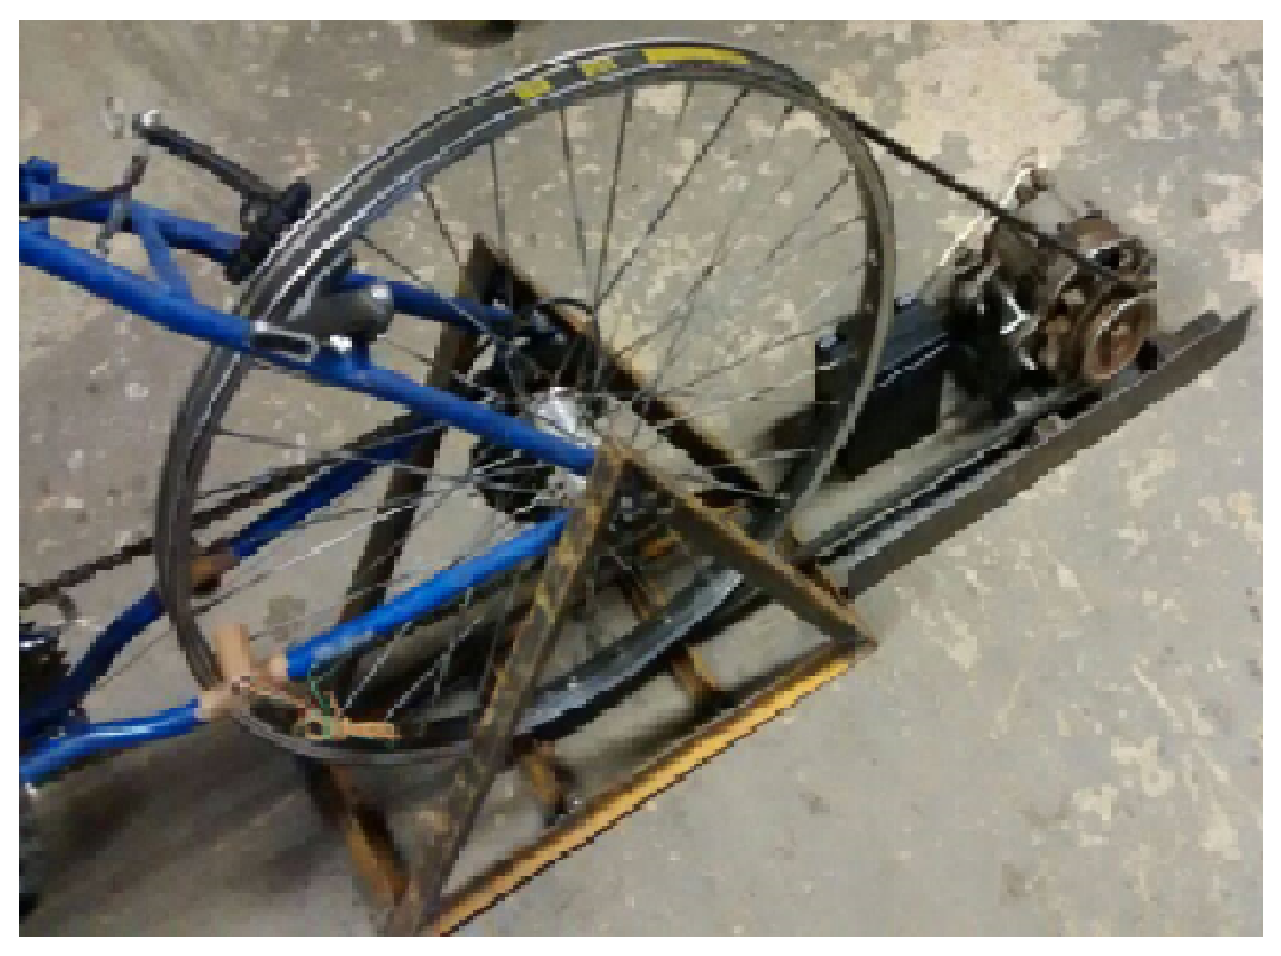
\includegraphics[width=0.5\textwidth]{figuras/image2}
  \caption{Sistema de transmissão de potência do Projeto START X: conexão entre polia motora e polia movida.}
  \label{sistema-transmissao}
\end{figure}

\subsubsection{Cálculo da potência mecânica no Projeto START X.}
\label{calculo-da-potencia-mecanica}

A potência mecânica de um corpo pode ser escrita da seguinte forma:

\begin{equation}
  Em={\frac{mv^{2}}{2}}\left ( w \right )  
  \label{potencia-mecanica}
\end{equation}

Onde:

\begin{itemize}
  \item Em=energia mecânica
  \item m=massa do corpo 
  \item v=velocidade do corpo
\end{itemize}

Apesar de muito útil a equação acima não consegue descreve a potência mecânica de um corpo quando este está fazendo um movimento circular. A equação a seguir mostra de outra forma como obter a potência mecânica.

\begin{equation}
  Em=\frac{Iw^{2}}{2}\left ( w \right )
\label{potencia-mecanica-circular}
\end{equation}

Onde:

\begin{itemize}
  \item I=momento de inércia do corpo 
  \item w=velocidade angular do mesmo
\end{itemize}

\subsubsection{Multímetro}

A potência mecânica que será entregue no eixo do gerador será convertida em energia elétrica, conforme já mencionado nesse relatório. Os aspectos físicos envolvidos na multicitada conversão foram detalhados na seção \ref{calculo-da-potencia-mecanica}, restando agora explicar como será a quantificação do resultado dessa conversão, isto é, quanto de energia elétrica será disponibilizado nos terminais do gerador.  Desse modo, para a suscitada quantificação, será colocado um multímetro digital (Figura \ref{multimetro}) na posição de leitura de potência, sendo que o mesmo será posicionado na saída dos terminais do gerador.

\begin{figure}
  \centering
  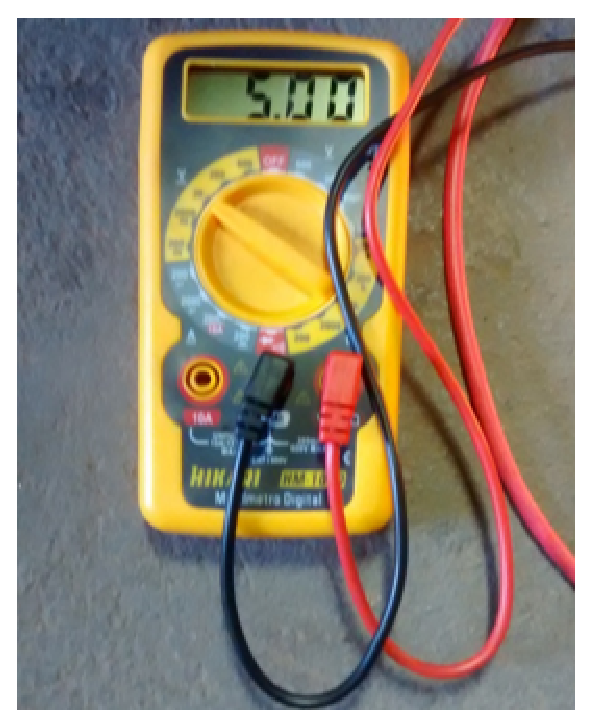
\includegraphics[width=0.4\textwidth]{figuras/image3}
  \caption{Multímetro digital utilizado no Projeto Start X.}
  \label{multimetro}
\end{figure}

\subsubsection{Cálculo da Potência Elétrica}

A potência elétrica pode ser obtida pela seguinte equação:

\begin{equation}
  Pe=V\ast I
  \label{potencia-eletrica}
\end{equation}

Onde:

\begin{itemize}
  \item Pe=potência elétrica
  \item V=tensão 
  \item I=corrente elétrica
\end{itemize}

Para o cálculo da potência elétrica consideramos que o usuário poderá gerar tensões entre 13 a 15 volts e correntes de 6 a 8,25 amperes sendo assim a potência elétrica gerada pelo sistema estará entre 78 e 123 watts para serem utilizados para a alimentação dos sensores e cargas de pequeno porte.

\subsubsection{Cálculo da Eficiência Energética}
\label{calculo-eficiencias-energeticas}

Uma vez calculadas as potências mecânica e elétrica, a próxima etapa consiste em quantificar a eficiência energética do processo de conversão eletromecânica do Projeto em tela. Para isso, as referidas potências serão relacionadas entre si conforme descrito na Equação \ref{efieciencia-energetica}.

\begin{equation}
\eta =\frac{P_{elet}}{P_{mec}}\left ( x \right )
\label{eficiencia-energetica}
\end{equation}

Onde: 

\begin{itemize}

  \item $\eta$ = eficiência energética
  \item $P_{elet}$= potência elétrica em Watt
  \item $P_{mec} $ = potência mecânica em Watt.
\end{itemize}

\subsubsection{Demonstração do Resultado da Eficiência Energética ao Usuário do Projeto Start X}

Como continuidade do presente projeto no futuro, sugere-se o aperfeiçoamento do sistema de conversão eletromecânico ligado à bicicleta, tanto em eficiência como funcionalidade. Com os dados obtidos durante a pedalada de potência mecânica e potência elétrica, pode-se obter a eficiência energética. 

Para demonstrar a eficiência energética ao usuário, serão coletados os dados das potências através de sensores futuramente instalados no pedal da bicicleta, para a potência mecânica, e os dados provenientes da medição através do multímetro, para a potência elétrica. Como mostrado anteriormente, a eficiência é dada pela divisão entre as duas potências obtidas. Pretende-se mostrar para o usuário a eficiência energética em cada uma das vezes que completar um circuito pedalado. Espera-se que essa eficiência varie de acordo com o tipo físico do usuário, o tipo do circuito, a velocidade e principalmente a frequência de pedalagem, que influencia diretamente o valor da potência mecânica.

\subsection{Dados do usuário}

O estudo ergonômico analisa principalmente as condições de trabalho em que as pessoas estão submetidas ao realizar uma atividade. Por exemplo, quando um motorista está ao volante, executa atividades corporais tão intensas quanto à de um operário em seu posto de trabalho. O corpo do motorista está submetido a esforços da posição de pilotagem e das forças transmitidas ao veículo. 

Para o desenvolvimento de projetos de produtos ergonômicos faz-se necessária a aplicação correta das dimensões humanas. Hoje a evolução das formas de análise de dados estatísticos aperfeiçoa as informações levantadas em uma pesquisa de dados antropométricos. Analises realizada ultimamente indicam que se um produto for dimensionado utilizando o manequim de 95\%  masculino e um manequim 5\% feminino este será capaz de acomodar 90\% da população escolhida. 
